\section{Design Model}


%%%%%%%%%%%%%%%%%%%%%%%%%%%%%%%%%%%%%%%
\subsection{Components and Overall Structure}
Structural design model.
see \ref{fig:dm:modules}. Application is in Java. Knowledge mostly in Jess and
for a part in Java (see section on inferences). Java application starts jess
engine with working memory.

In the working memory are the domain rules, facts
that represent inferential knowledge of car, and the domain parts, knowledge
about the current status of parts of the car. Domain rules are not modified over
a run of the program, domain parts are modified.

Information from the app goes to jess by asserting
support facts, these are then interpeted as modifications of domain parts.
Inferences made by Jess go to the app by queries made by the app.

The Jess parts is divided in a engine and a domain part. The domain rules and
domain parts are implementations of templates supplied by the engine. The
engines inferences makes forward and backward reasonings from these rules and
parts. The domain rules and parts can be substituted by rules and parts from a
different domain while keeping the engine. The rules might be understandable by an
expert or user, our car repair hobbyist does. The complexity of the inferences
made by the engine are not visible in the domain part.

\begin{figure}[htbp]
    \centering
    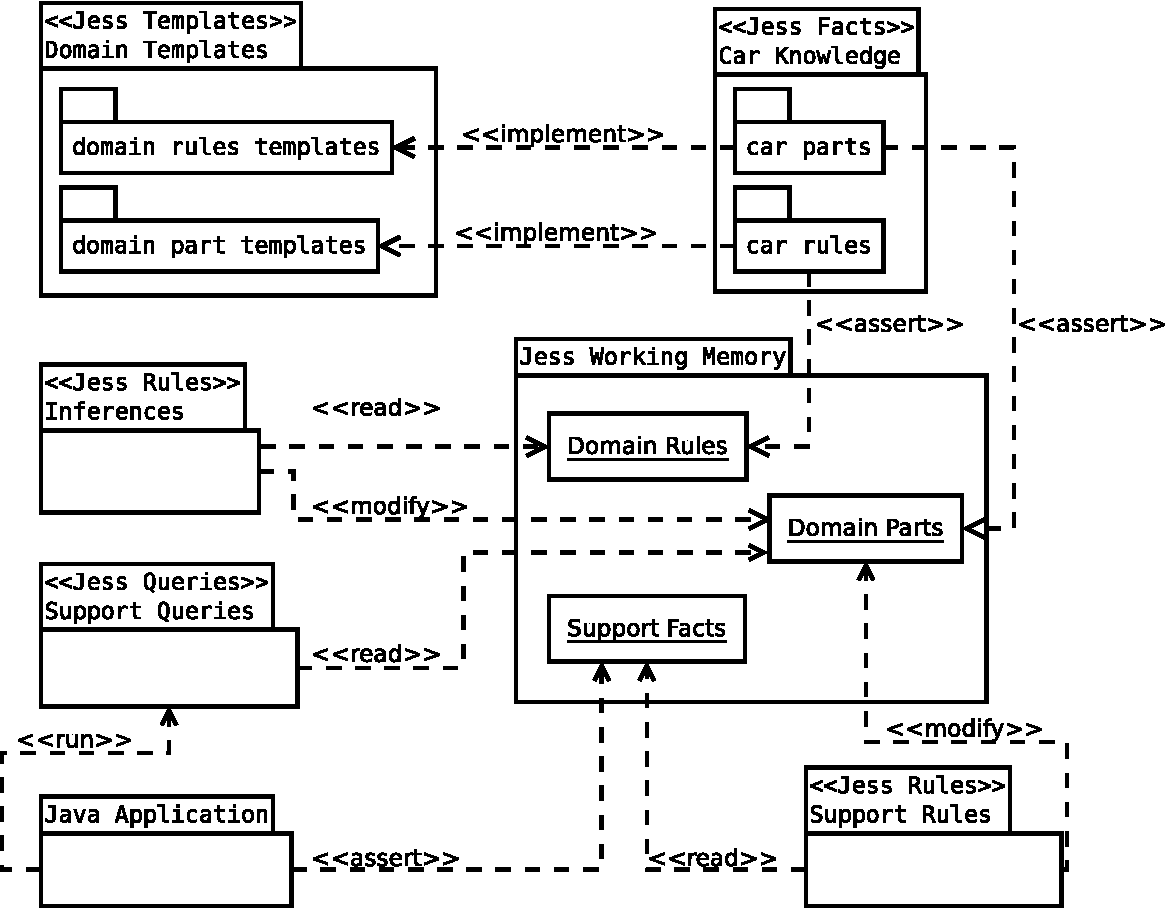
\includegraphics[width=1.00\textwidth]{dm-modules}
    \caption{The modular structure of the design model}
    \label{fig:dm:modules}
\end{figure}

%%%%%%%%%%%%%%%%%%%%%%%%%%%%%%%%%%%%%%%
\subsection{The process flow}
The overall flow of the application can be seen in the activity diagram in
figure~\ref{fig:dm:activity diagram}. It implements the communication, as
modelled in figure~\ref{fig:communicationPlan}, and the task method, as seen in
figure~\ref{fig:taskMethod}.

The process start when a complaint is reported to the system. The system then covers
all hypothesis that follow from the complaint. The rest of the process is one
big loop. It has two exits, when a succesfull repair is made, and when there are
no viable hypothesis left. Inside the loop, first, a hypothesis is selected with
user assistance. Secondly an attempt is made to make an observation. This is a
loop where the user is asked to observe all the possible observables on after
another. If the user want do do an observation the result is used to update the
hypothesis in the verify activity. If the user doesn't want do to any of the
observations or there are no observables for the hypothesis, the user is asked
to repair his or her car. If this repair is succesfull the problem is solved and
the program exits. If the repair isn't succesfull, the hypothesis is deemed
impossible by the system.

\begin{figure}[htbp]
    \centering
    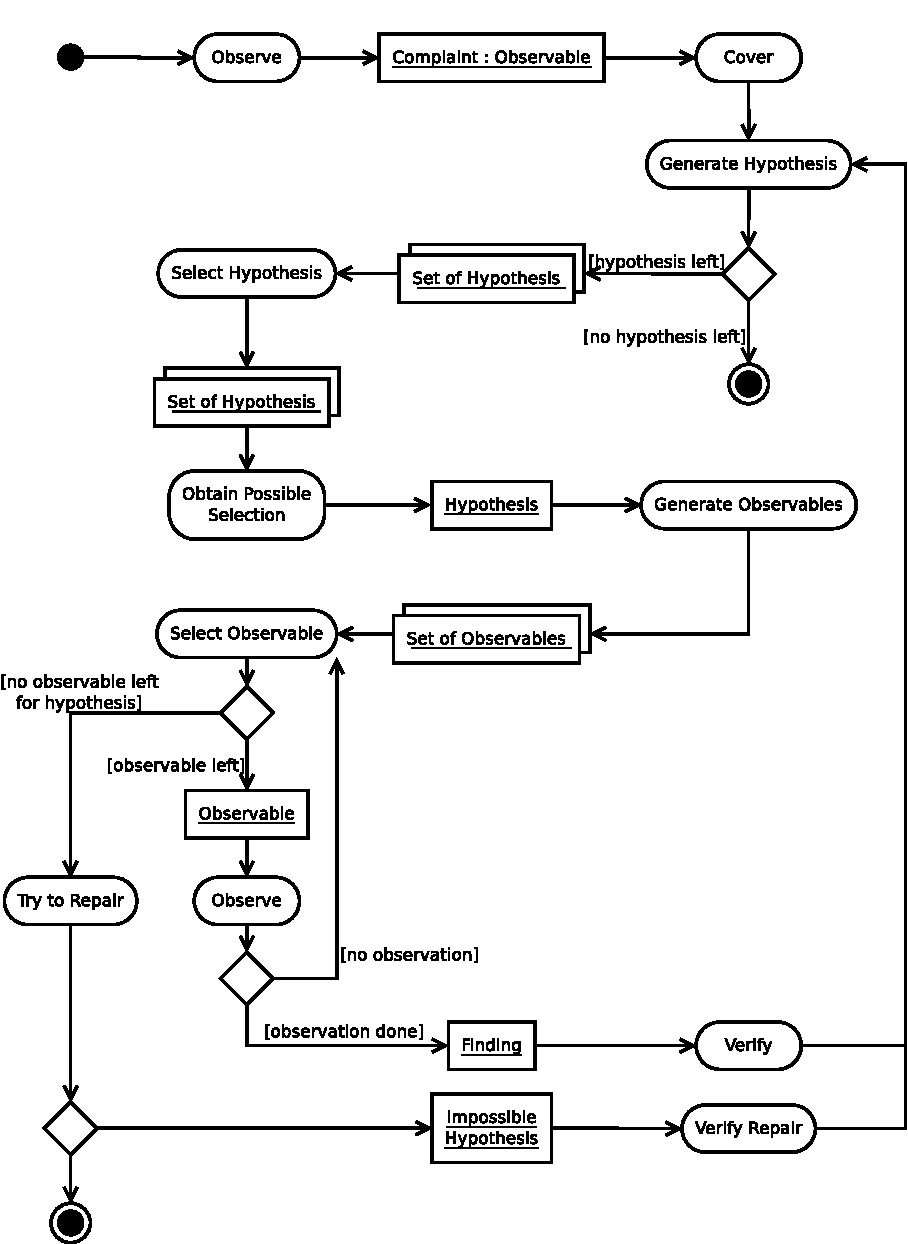
\includegraphics[width=1.00\textwidth]{dm-activity}
    \caption{The overal activity diagram of the application}
    \label{fig:dm:activity diagram}
\end{figure}

%%%%%%%%%%%%%%%%%%%%%%%%%%%%%%%%%%%%%%%
\subsection{The application}
class diagram in figure~\ref{fig:dm:class diagram}. %TODO
\begin{figure}[htbp]
    \centering
    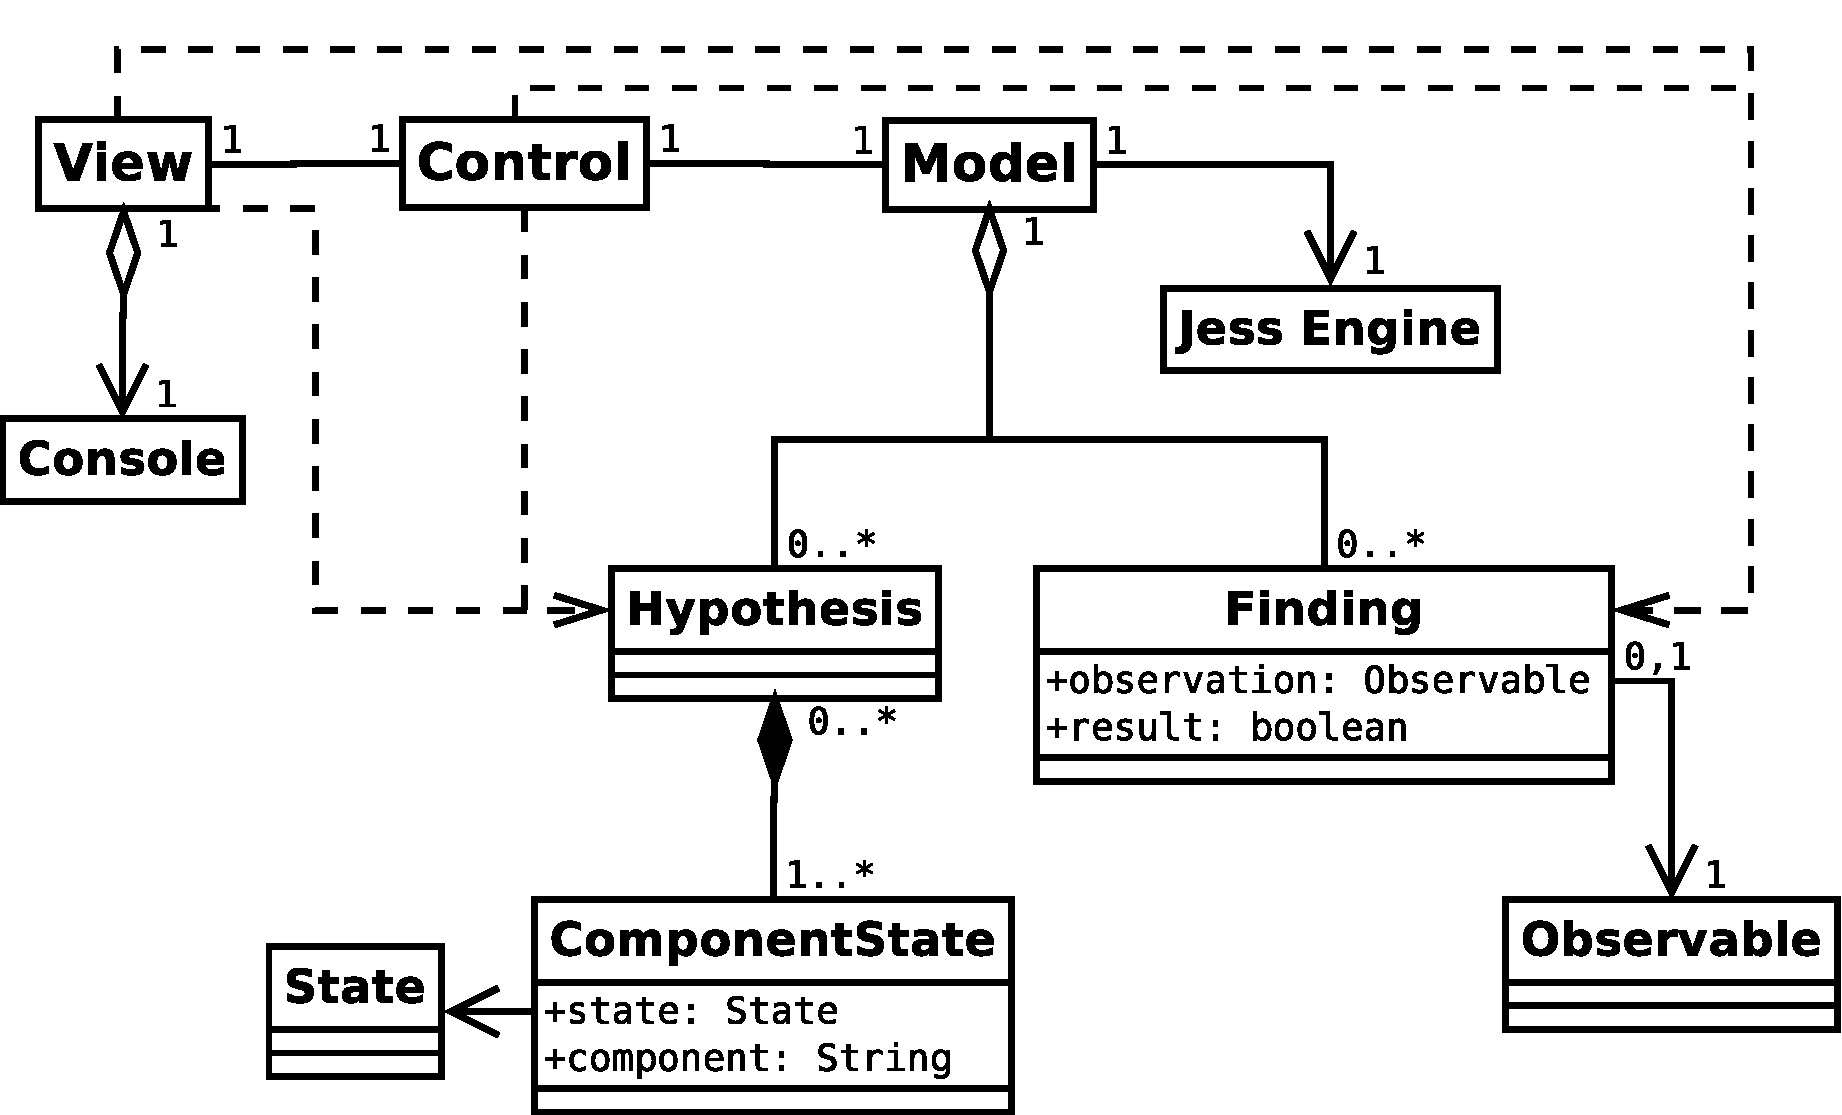
\includegraphics[width=1.00\textwidth]{dm-class}
    \caption{The class diagram of the Java application}
    \label{fig:dm:class diagram}
\end{figure}

The model-view-controller pattern is applied. The model keeps all the knowledge
of the system. The Java class is partly an interface to the part of the model
that is implemented in Jess and partly implements the knowledge of the model
itself, as explained in the next section. The control manages the process flow,
as described in the previous section, and communicates with the model and the
view components. The view implements the user interface and the part of the user
interaction that doesn't involve the model.

The activity diagram of figure~\ref{fig:dm:activity diagram} is further detailed
in three state diagrams showing the communication between the model, view and
controller components. The first diagram, in figure~\ref{fig:dm:sd cover}, %TODO
The second diagram, in figure~\ref{fig:dm:sd select}, %TODO
The third diagram, in figure~\ref{fig:dm:sd observe}, %TODO

\begin{figure}[htbp]
    \centering
    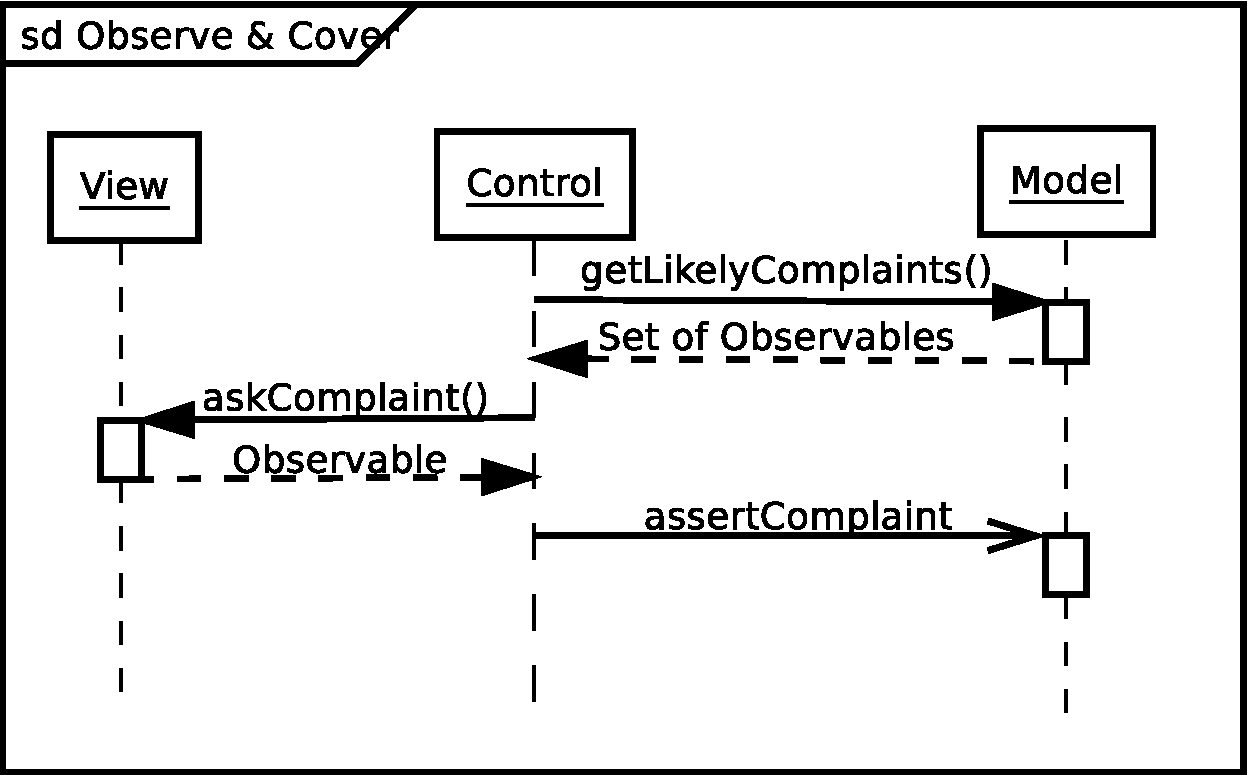
\includegraphics[width=1.00\textwidth]{dm-sd-cover}
    \caption{The state diagram detailing report and cover}
    \label{fig:dm:sd cover}
\end{figure}

\begin{figure}[htbp]
    \centering
    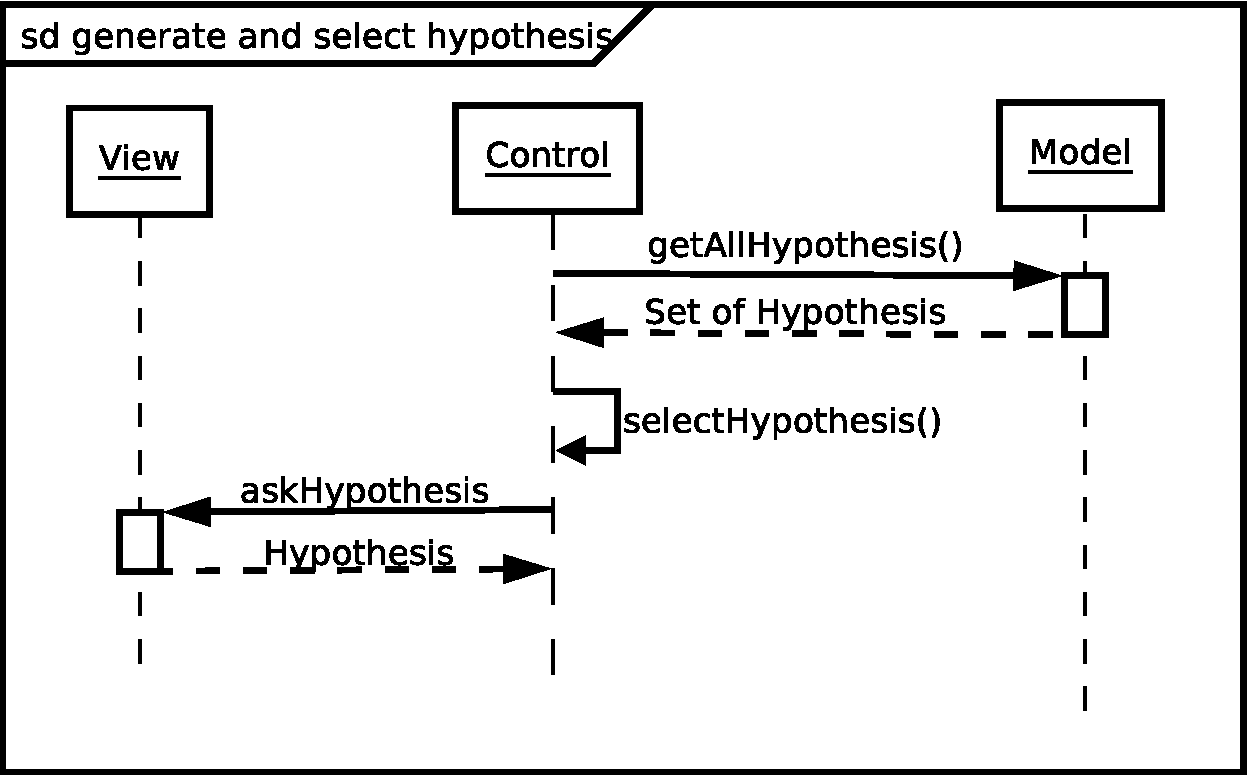
\includegraphics[width=1.00\textwidth]{dm-sd-select}
    \caption{The state diagram detailing generating and selecting hypothesis}
    \label{fig:dm:sd select}
\end{figure}

\begin{figure}[htbp]
    \centering
    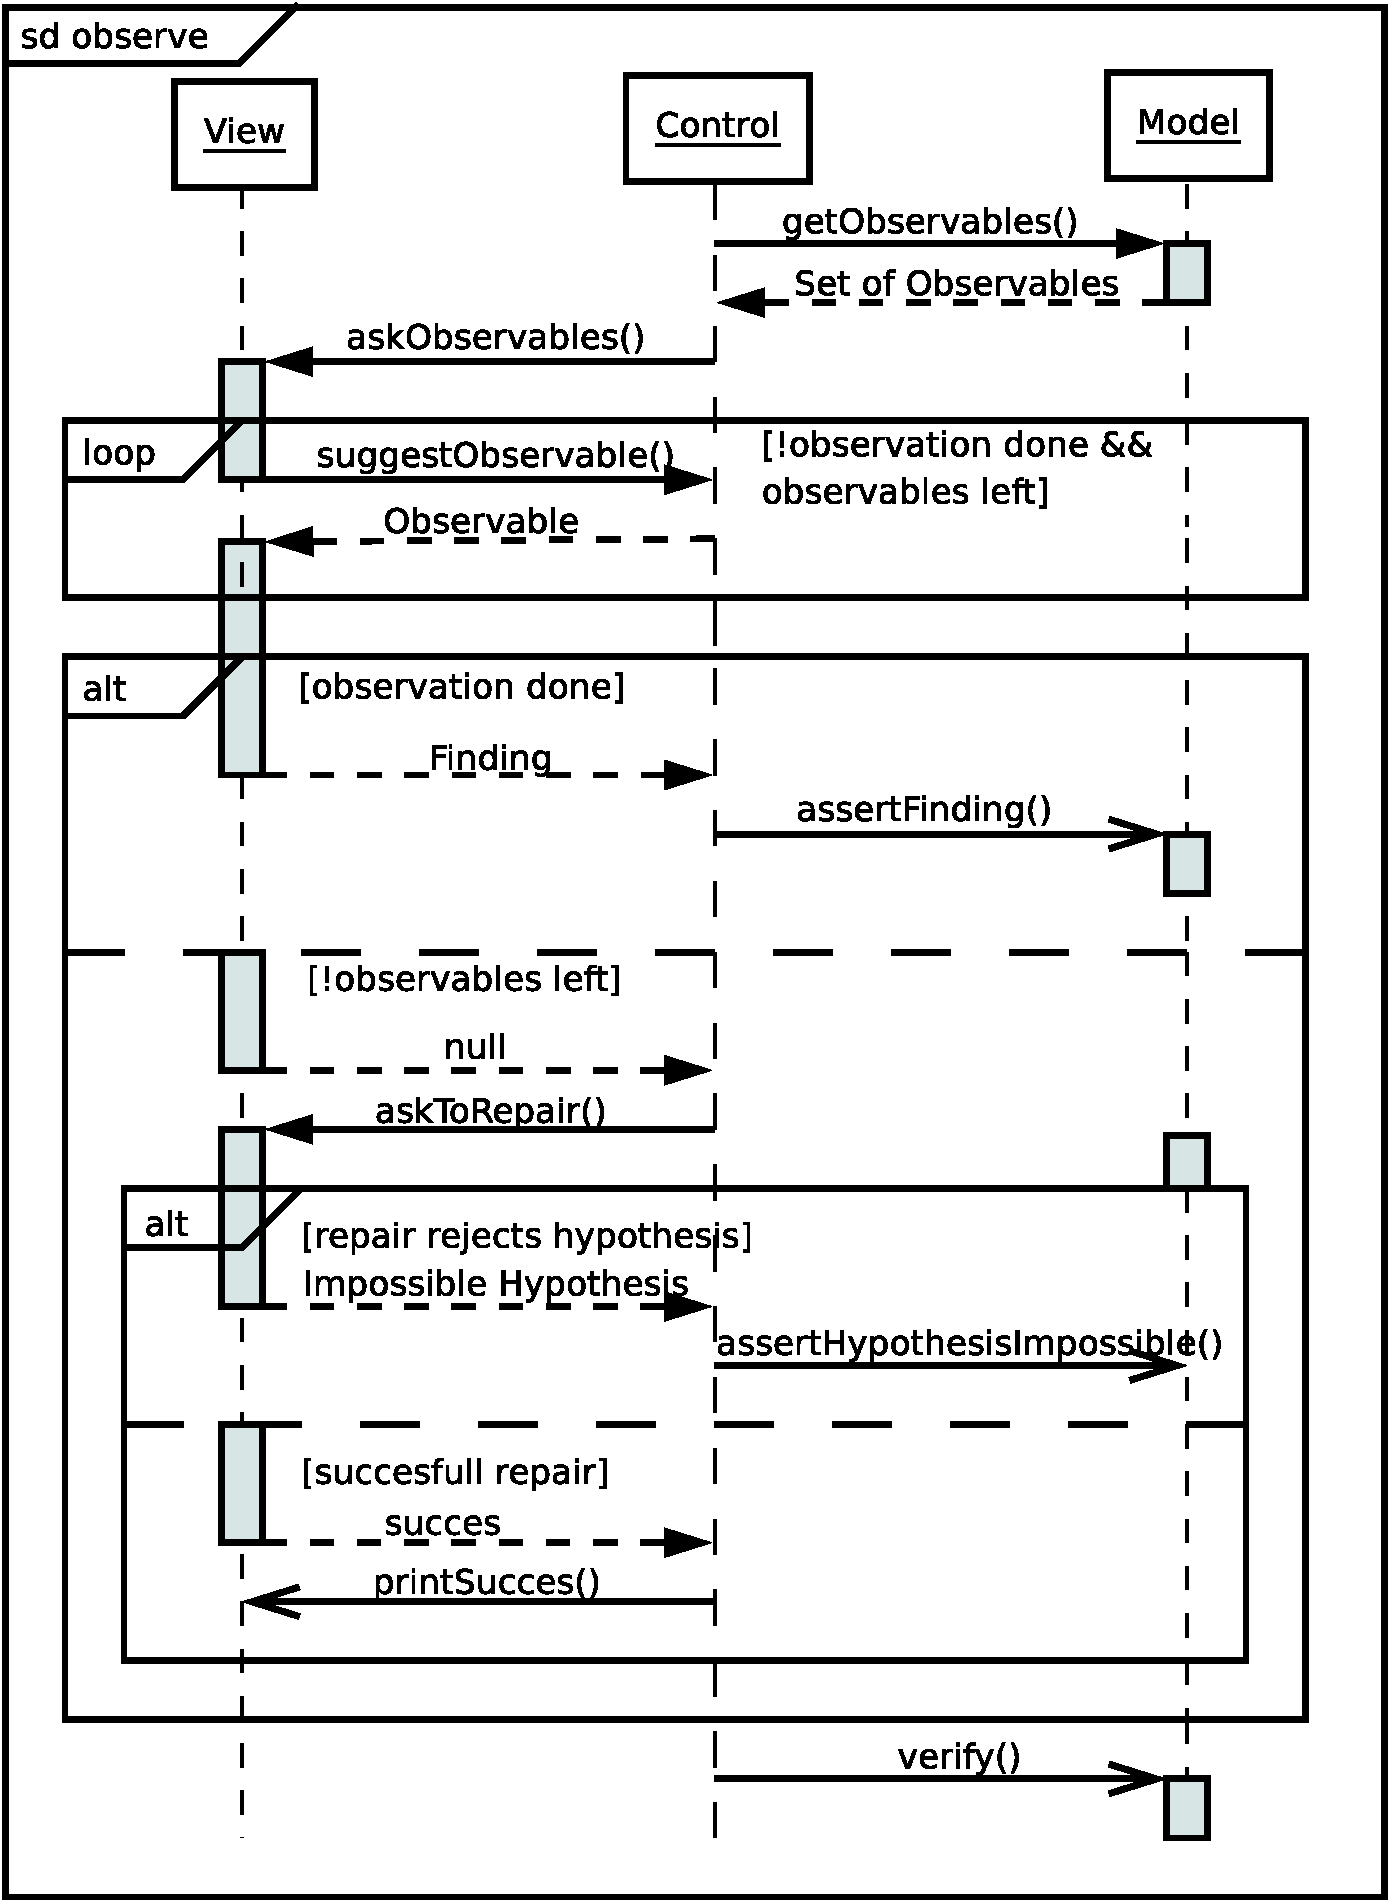
\includegraphics[width=1.00\textwidth]{dm-sd-observe}
    \caption{The state diagram detailing observations, try to repair and verify}
    \label{fig:dm:sd observe}
\end{figure}
